In this Chapter we compare performances of our method against a number of different baselines on a
series of different problems. The algorithms we compare against are POMCP, RTBSS and a belief based
RTBSS (which we refer to as RTBSSb).

RTBSS is an online branch-and-bound solver for POMDPs, which enumerates every possible outcome from
a given state for a given horizon, and thus computes the true value function for that state and the
best action that can be performed. RTBSSb works in the same way, but it computes rewards using a
given belief-based reward function. RTBSS trades its precision and accuracy with speed: since it has
to explore most of the possible outcomes, the size of problems it can handle is limited.

Even though POMCP and RTBSS are algorithms which require a state-based reward function, we can
compare them against the performance of max-of-belief $\rho$-POMCP. This is possible since a
max-of-belief reward function can be converted into a state-based reward function by modifying the
action space of the problem \cite{cit:rpomdp}. In the new action space, each action represents at
the same time one of the old actions, plus an addictional \textit{prediction action}, which is used
by the agent in order to predict the state the environment is in at any given time. The new action
space is thus the result of a cross-product between the set of old actions and the new prediction
actions, which are $|S|$.

% \ys{be consistent with the framework you are using. Stick to rho POMDP, no need for prediction
% actions}
%
% Well, my approach does not need prediction actions, but POMCP and RTBSS do need it. Since I spent
% all the thesis outlining why POMCP could not be used, it makes sense to give an outline to it, or
% no?

The reward function is then defined in terms of the prediction actions: if the agent predicts the
state of the environment correctly, it receives a reward of 1. Otherwise, it receives no reward. It
follows that the expected returns with the new reward function are the same than that of a
max-of-belief reward function, as the agent will guess the state of the environment correctly with a
rate equal to the maximum of its belief.

The disadvantage of this transformation is that the action space becomes exponentially bigger the
more states are available, which significantly impairs both POMCP and RTBSS.

RTBSSb can instead be applied directly on both max-of-belief and entropy based rewards, but still
has to explore the action-observation tree in order to select the best action.

\section{First Model - Simple Environment}

In this section we apply the proposed algorithms to the following model: a single target walking
between six rooms. The target can be at any time in a single room, and can transition between them
as showed in \ref{ref:nonmyo1}. The agent can observe, at each timestep, whether the target is in a
given room. The information gathered by the agent will be correct with probability $p=0.8$. In each
episode the target starts in a random room, and the agent goal is to track it for 10 timesteps. The
agent receives a reward of 1 if it can correctly guess the position of the target, and 0 otherwise.
This problem is also discussed in Appendix \ref{ref:appendix_proof} to show how a non-myopic
approach can be preferred over a myopic one.

It is important to note that this reward scheme thus strongly favors the max-of-belief reward
function over entropy, since the two functions maximize different things: max-of-belief will use its
resources to try and determine the target's position with absolute certainty at the expense of
general knowledge, while entropy will try to determine the target's general area but ignoring the
details. So the methods using entropy will most probably obtain on average less reward than the ones
using max-of-belief.


\begin{figure}[ht!]
\centering
\begin{tikzpicture}[->,>=stealth',shorten >=1pt,auto,node distance=4cm,thick,main node/.style={circle,draw,font=\Large\bfseries}]
\tikzstyle{state} = [circle, draw=black, fill=green!30]
\tikzstyle{arrow} = [thick,->,>=stealth]

\node (s1) at (0,0) [state] {S1};
\node (s2) at (2,3) [state] {S2};
\node (s3) at (4,0) [state] {S3};
\node (s4) at (6,0) [state] {S4};
\node (s5) at (8,3) [state] {S5};
\node (s6) at (10,0) [state] {S6};

\path
    (s1) edge [loop below] node {0.333} (s1)
         edge [bend left] node {0.333} (s2)
         edge [bend left=10] node[below] {0.333} (s3)
    (s2) edge [loop above] node {0.333} (s2)
         edge [bend left=10] node[above,rotate=60] {0.333} (s1)
         edge [bend left] node {0.333} (s3)
    (s3) edge [loop below] node {0.333} (s3)
         edge [bend left=10] node[above,rotate=-60] {0.333} (s2)
         edge [bend left] node {0.333} (s1)
    (s4) edge [bend left] node {1.0} (s5)
    (s5) edge [bend left] node {1.0} (s6)
    (s6) edge [bend left] node {1.0} (s4);

\end{tikzpicture}
\caption{The graphical representation of our first model.}
\label{ref:nonmyo1}
\end{figure}

Figure \ref{ref:myoentropyfig} shows performance in terms of cumulative obtained reward for the
different methods proposed. The $h$ parameter determines the horizon of the particular solver. $h =
1$ results in a greedy solver. It is important to note that for POMCP and $\rho$-POMCP $h$ is merely an
upper bound on the depth of the decision tree they are allowed to explore. This is because they
build their decision tree incrementally, so that they may not reach the true bottom of their
decision tree if the number of samples is not sufficient. This most often happens for POMCP since
the technique used to apply it to Active Perception substantially increases the branching factor of
the decision tree.

\begin{figure}[ht!]
        \centering
        \begin{subfigure}[t]{0.45\textwidth}
                \includegraphics[width=\textwidth]{Images/MyoResults/1e4/E/output}
                \caption{Results using 1e4 samples, with entropy as the reward function.}
                \label{fig:m4e}
        \end{subfigure}%
        ~ %add desired spacing between images, e. g. ~, \quad, \qquad, \hfill etc.
          %(or a blank line to force the subfigure onto a new line)
        \begin{subfigure}[t]{0.45\textwidth}
                \includegraphics[width=\textwidth]{Images/MyoResults/1e4/MB/output}
                \caption{Results using 1e4 samples, with max-of-belief as the reward function.}
                \label{fig:m5e}
        \end{subfigure}
        \caption{Results in our first model, averaged over 3000 episodes.}
        \label{ref:myoentropyfig}
\end{figure}

We can see how a small horizon always results in a lower return over the 10 timesteps. This is
because with a greedy approach the agent cannot leverage the fact that half of the environment is
deterministic, and thus more useful to explore beforehand. This is most visible in the max-of-belief
setting, while the entropy reward function does not suffer from a significant loss of performance.
In addition, we can see how POMCP does not improve even with a larger horizon, probably due to being
incapable of exploring the decision tree in great depth with its available samples.

\section{Second Model - Finite Budget}

In this Section we apply the proposed algorithms to the following model: a 4-room world where a
target can transition, at each timestep, from a room to any of the two rooms adjacent. The
observation and reward function follow the logic of our first model: the agent can observe a single
room at a time, and needs to keep track of the target for 15 timesteps. The target here always
starts from a given room, known to the agent.

In this model there is an additional rule: the agent is only allowed to look at the world 4 times;
after that each action will yield no additional information. The agent can, at each timestep, decide
whether to use one of its observations, or save them for a future timestep. This last constraint is
used to simulate real-life resource constraints; for example when energy and/or processing
constraints limit the number of times a multi-camera system is allowed to observe the environment.

The idea is that the agent should use up an observation only if has low knowledge about the world;
otherwise it should keep its observation actions for later and try to extract as much reward from
current knowledge as possible.

\begin{figure}[ht!]
\centering
\begin{tikzpicture}[->,>=stealth',shorten >=1pt,auto,node distance=4cm,thick,main node/.style={circle,draw,font=\Large\bfseries}]
\tikzstyle{state} = [circle, draw=black, fill=green!30]
\tikzstyle{arrow} = [thick,<->,>=stealth]

\node (s1) at (0,3) [state] {S1};
\node (s2) at (3,3) [state] {S2};
\node (s3) at (0,0) [state] {S3};
\node (s4) at (3,0) [state] {S4};

\path
    (s1) edge [arrow] node {0.5} (s2)
    (s2) edge [arrow] node {0.5} (s4)
    (s3) edge [arrow] node {0.5} (s1)
    (s4) edge [arrow] node {0.5} (s3);

\end{tikzpicture}
\caption{The graphical representation of our second model.}
\label{ref:finbudget1}
\end{figure}

We tested this model in two configurations: one where the target transitions randomly between the
two rooms available, increasing maximally the entropy at each timestep, and one where the target
transitions to its left with a probability of $0.75$. This was done in order to see how the agent behavior
changed with respect to a differently predictable target.

\begin{figure}[ht!]
        \centering
        \begin{subfigure}[t]{0.45\textwidth}
                \includegraphics[width=\textwidth]{Images/FiniteBudgetResults/0.5/1e4/E/output}
                \caption{Results using 1e4 samples, and entropy as the reward function.}
                \label{fig:fb4e5}
        \end{subfigure}%
        ~ %add desired spacing between images, e. g. ~, \quad, \qquad, \hfill etc.
          %(or a blank line to force the subfigure onto a new line)
        \begin{subfigure}[t]{0.45\textwidth}
                \includegraphics[width=\textwidth]{Images/FiniteBudgetResults/0.5/1e4/MB/output}
                \caption{Results using 1e4 samples, and max-of-belief as the reward function.}
                \label{fig:fb5e5}
        \end{subfigure}
        \caption{Results in the Finite Budget model with a transition factor of 0.5, averaged over 3000 episodes.}
        \label{ref:fbentropyfig5}
\end{figure}

In Figure \ref{ref:fbentropyfig5} we can see how always looking seems to be the best choice for the
agent, if the uncertainty about the target is too high to risk losing it even for a brief time.
Thus, the agent always uses all its resources as soon as it can in order to accrue as much reward as
possible. The myopic IR solvers however seem to have trouble even with this concept, as they do not
see the advantage of using their resources, instead focusing simply on the prediction action for the
current timestep.

\begin{figure}[ht!]
        \centering
        \begin{subfigure}[t]{0.45\textwidth}
                \includegraphics[width=\textwidth]{Images/FiniteBudgetResults/0.75/1e4/E/output}
                \caption{Results using 1e4 samples, and entropy as the reward function.}
                \label{fig:fb4e75}
        \end{subfigure}%
        ~ %add desired spacing between images, e. g. ~, \quad, \qquad, \hfill etc.
          %(or a blank line to force the subfigure onto a new line)
        \begin{subfigure}[t]{0.45\textwidth}
                \includegraphics[width=\textwidth]{Images/FiniteBudgetResults/0.75/1e4/MB/output}
                \caption{Results using 1e4 samples, and max-of-belief as the reward function.}
                \label{fig:fb5e75}
        \end{subfigure}
        \caption{Results in the Finite Budget model with a transition factor of 0.75, averaged over 3000 episodes.}
        \label{ref:fbentropyfig75}
\end{figure}

In Figure \ref{ref:fbentropyfig75} we see how payouts increase slightly due to the target being more
predictable; but once again the best choice seems to avoid losing track of the target rather than
guessing and then finding it again. This is surprising, given the small size of the environment,
since the agent should be driven to guessing if the chance it can actually lose the target is low.

\section{Third Model - Realistic Scenario}

In this Section we test $\rho$-POMCP on yet another model. Here the target can walk in a grid world,
in a north-south-east-west fashion. To produce a somewhat realistic environment, the target selects
a random cell at any time, and then moves towards it. Once it reaches it, it selects another goal
cell, and continues. However, the agent's model of the environment does not include this: the agent
only knows that the target can move randomly towards an adjacent cell. The target always starts from
the center of the grid, with the agent knowing it.

The world is observed by cameras, where each camera can observe a 5x5 patch of the overall world,
with no overlap. Each camera can observe imperfectly: the closer the target is towards the center
of the patch, the more accurate the observations will be. Otherwise the camera will observe the
target on any cell adjacent to the true target. If the adjacent cell is outside the camera range,
the camera will not see the target.

The agent is allowed to use a single camera at the time, and needs to keep track of the target over
75 timesteps.

We show results with two different versions of the world: a small 20x20 environment, and a bigger
50x50 one. Due to the big number of states, POMCP and RTBSS cannot be used here; RTBSSb can be
barely used with a greedy horizon for the small environment.

\begin{figure}[ht!]
        \centering
        \begin{subfigure}[t]{0.45\textwidth}
                \includegraphics[width=\textwidth]{Images/CameraBasicResults/Small_20x20/1e4/output}
                \caption{Results using 1e4 samples.}
                \label{fig:cws4mb}
        \end{subfigure}%
        ~ %add desired spacing between images, e. g. ~, \quad, \qquad, \hfill etc.
          %(or a blank line to force the subfigure onto a new line)
        \begin{subfigure}[t]{0.45\textwidth}
                \includegraphics[width=\textwidth]{Images/CameraBasicResults/Big_50x50/1e4/output}
                \caption{Results using 1e5 samples.}
                \label{fig:cws5mb}
        \end{subfigure}
        \caption{Results in our realistic model using a 20x20 grid averaged over 3000 episodes.}\label{fig:cwsmb}
\end{figure}

The results in Figure \ref{fig:cws5mb} show that there does not seem a particular advantage in
non-myopic planning. This is probably due to the very high symmetry of the environment. Since every
direction that could be taken by the target would lead them into a new position with pretty much the
same possible future development (aside from the edges of the grid), future expectations are
necessarily mirrored no matter what the target does. This makes planning in the future not really
useful.

In Figure \ref{fig:cwb10} we show the results of applying $\rho$-POMCP to a multi-tracking scenario, where
10 targets are allowed to roam the grid world concurrently. In this experiment, we run 10 instances
of $\rho$-POMCP in a parallel fashion, one for each target. These 10 instances approximate values for
every possible action, given their belief on their respective target. At every timestep, the action that
maximizes overall value over all $\rho$-POMCP instances is chosen.

\begin{figure}[ht!]
        \centering
        \begin{subfigure}[t]{0.5\textwidth}
                \includegraphics[width=\textwidth]{Images/CameraBasicResults/Big_50x50/Multi/E/output}
                \caption{Results using 1e4 samples and entropy.}
                \label{fig:cwb4e10}
        \end{subfigure}%
        ~ %add desired spacing between images, e. g. ~, \quad, \qquad, \hfill etc.
          %(or a blank line to force the subfigure onto a new line)
        \begin{subfigure}[t]{0.5\textwidth}
                \includegraphics[width=\textwidth]{Images/CameraBasicResults/Big_50x50/Multi/MB/output}
                \caption{Results using 1e4 samples and max-of-belief.}
                \label{fig:cwb5mb10}
        \end{subfigure}
        \caption{Results in our realistic model 50x50 tracking 10 unique targets, averaged over 3000 episodes.}
        \label{fig:cwb10}
\end{figure}

With multiple targets the behavior of the agent started to differ significantly whether we used the
entropy reward function or the max-of-belief reward function.

With the entropy reward function the agent tried to follow all targets equally, exploring the
environment when targets were lost too much, trying to always have some idea of where each target
was. This could be the reason why in Figure \ref{fig:cwb4e10} we see that planning with an horizon
of 5 seems to give slightly better results.

On the other hand, the max-of-belief reward function focused on keeping close track of a subset of
targets, preferring to avoid losing resources into keeping track of targets whose position was not
precisely known. This behavior allows the agent to get a high reward in terms of the number of
targets exactly tracked, at the expense of completely losing tracks of other targets.

\subsection{Realistic Scenario with Movement Prediction}

In addition to the previous experiments, we also created a separate model where the agent's model of
the target movements is improved. In this second version of Camera World, the model keeps track of
the previous direction that the target moved, and predicts a $0.7$ probability that the target will
continue to move in the same direction, or randomly otherwise. This is done by increasing the state
space by four times, where each state now encodes a previous target direction and the target current
position.

In this new model unfortunately RTBSSb cannot be used, as the state space is too big and RTBSSb
takes too much time to complete.

\begin{figure}[ht!]
        \centering
        \begin{subfigure}[t]{0.45\textwidth}
                \includegraphics[width=\textwidth]{Images/CameraPathResults/Small_20x20/1e4/output}
                \caption{Results using 1e4 samples.}
                \label{fig:cps4e}
        \end{subfigure}%
        ~ %add desired spacing between images, e. g. ~, \quad, \qquad, \hfill etc.
          %(or a blank line to force the subfigure onto a new line)
        \begin{subfigure}[t]{0.45\textwidth}
                \includegraphics[width=\textwidth]{Images/CameraPathResults/Big_50x50/1e4/output}
                \caption{Results using 1e5 samples.}
                \label{fig:cps5e}
        \end{subfigure}
        \caption{Results in the Camera World 2 20x20, using entropy, averaged over 3000 episodes.}
        \label{fig:cpse}
\end{figure}

In Figure \ref{fig:cpse} we see once again that non-myopic planning seems to be wasted in terms of
added value, when we track a single target in a highly symmetric environment.

\begin{figure}[ht]
        \centering
        \begin{subfigure}[t]{0.5\textwidth}
                \includegraphics[width=\textwidth]{Images/CameraPathResults/Big_50x50/Multi/E/output}
                \caption{Results using 1e4 samples and entropy.}
                \label{fig:cpb4e10}
        \end{subfigure}%
        ~ %add desired spacing between images, e. g. ~, \quad, \qquad, \hfill etc.
          %(or a blank line to force the subfigure onto a new line)
        \begin{subfigure}[t]{0.5\textwidth}
                \includegraphics[width=\textwidth]{Images/CameraPathResults/Big_50x50/Multi/MB/output}
                \caption{Results using 1e4 samples and max-of-belief.}
                \label{fig:cpb5mb10}
        \end{subfigure}
        \caption{Results in the Camera World 2 50x50 tracking 10 unique targets, averaged over 3000 episodes.}\label{fig:cpb10}
\end{figure}

In Figure \ref{fig:cpb10} we discover a particular behaviour of the max-of-belief reward function:
it seems to perform much better with myopic planning rather than with non-myopic planning, which
generally should not happen - performances of both approaches should in the worst case be equal.

This happens due to our implementation of multi-target tracking. Each planner is planning for a
single target, completely ignoring the rest. Thus, non-myopic planning results in many parallel
planners trying to discover the best actions in order to maximise the reward for their target,
\textit{given that future actions will follow the policy they are planning}. In other terms, the
value of each action given by each planner assumes that future actions will follow that planner's
policy.

Since instead each action is chosen by summing all values given by each planners to that action,
future actions are not necessarily going to follow any particular planner's policy. Thus, non-myopic
planning is actually interfering with the planning phase, since it ends up assigning wrong values to
each action.
